\documentclass[11pt,a4paper]{article}
\usepackage[margin=0.8in]{geometry}
\usepackage{amsmath,amssymb}
\usepackage{graphicx}
\usepackage{hyperref}
\usepackage{booktabs}
\usepackage{enumitem}
\usepackage{tikz}
\usetikzlibrary{shapes.geometric, arrows, positioning, calc}
\usepackage{pgfgantt}
\usepackage{xcolor}
\usepackage{fancyhdr}
\usepackage{titlesec}

% Define custom colors for Gantt chart
\definecolor{phase1color}{RGB}{52, 152, 219}    % Blue
\definecolor{phase2color}{RGB}{46, 204, 113}    % Green
\definecolor{phase3color}{RGB}{241, 196, 15}    % Yellow
\definecolor{phase4color}{RGB}{231, 76, 60}     % Red

% Header and footer
\pagestyle{fancy}
\fancyhf{}
\rhead{Phase 1: Project Report}
\lhead{Postcondition Auditor}
\cfoot{\thepage}

% Section formatting
\titleformat{\section}{\large\bfseries}{\thesection}{1em}{}
\titleformat{\subsection}{\normalsize\bfseries}{\thesubsection}{1em}{}

\title{\textbf{The Postcondition Auditor: A Rigorous Analysis of LLM Prompting Strategies} \\ 
\large \textbf{Phase 1 Project Report} \\
Software Systems Development Course \\ 
IIIT Hyderabad}
\date{}

\begin{document}

\maketitle
\vspace{-1.5cm}
\begin{table}[h]
\centering
\begin{tabular}{@{}ll@{}}
\toprule
\multicolumn{2}{c}{\textbf{TEAM NO 32}} \\ \midrule
\textbf{NAME} & \textbf{ROLL NO} \\
\midrule
Naveen Mishra & 2025201084\\
Radha Krishna Nallagatla & 2025201069 \\
Vipin Yadav & 2025201013 \\
Sriram Puruchuri & 2025201074 \\
Mohd Shahid Kaleem & 2025204008 \\
\bottomrule
\end{tabular}
\caption{Team Details}
\end{table}

\section{Project Understanding and Scope}

\subsection{Problem Statement Analysis}
The Postcondition Auditor project addresses a critical challenge in automated software verification: \textbf{evaluating the effectiveness of Large Language Models (LLMs) in generating accurate and reliable postconditions}. This research initiative, conducted under the Software Engineering Research Centre (SERC) framework, moves beyond mere demonstration to provide quantifiable, evidence-based conclusions on LLM performance.

The core problem revolves around the \textbf{automated generation and evaluation of postconditions} - logical assertions that specify the expected state after function execution. Traditional manual verification approaches are time-intensive and error-prone, making LLM-assisted automation an attractive research direction. However, the reliability and accuracy of LLM-generated postconditions remain uncharted territory requiring systematic investigation.

\subsection{Research Objectives and Significance}
Our primary objective is to design a \textbf{novel evaluation framework} that conducts definitive comparative analysis of three distinct LLM prompting strategies:
\begin{itemize}[itemsep=0pt]
    \item \textbf{Naive Prompt}: Direct, zero-shot instruction approach
    \item \textbf{Few-Shot Prompt}: Incorporates three hand-curated exemplar postconditions
    \item \textbf{Chain-of-Thought (CoT) Prompt}: Explicit reasoning about function purpose, invariants, and edge cases
\end{itemize}

The significance lies in establishing \textbf{quantitative benchmarks} for LLM postcondition generation across three critical dimensions: correctness (validity), completeness (strength), and soundness (reliability). This research contributes to the broader field of automated software verification and LLM applications in software engineering.

\subsection{Dataset and Constraints}
The experiment utilizes a \textbf{curated subset of 50 functions} from the Most Basic Programming Problems (MBPP) dataset, each accompanied by function signatures, implementations, and comprehensive input-output test cases. This dataset provides sufficient complexity while maintaining experimental manageability within our 8-week timeline.

\section{Team Composition and Persona Analysis}

\subsection{Team Structure and Philosophy}
Our 5-member team adopts an \textbf{independent responsibility model} designed to maximize parallel development and minimize inter-dependencies. Each team member will assume primary ownership of a distinct project component while maintaining collaborative oversight of the overall system architecture.

\subsection{Proposed Responsibility Matrix}
\begin{table}[h]
\centering
\begin{tabular}{@{}ll@{}}
\toprule
\textbf{Team Member} & \textbf{Primary Responsibility} \\
\midrule
Naveen Mishra & LLM Integration \& Prompting Strategy Implementation \\
Radha Krishna Nallagatla & Property-Based Testing \& Correctness Evaluation \\
Vipin Yadav & Mutation Analysis \& Completeness Assessment \\
Sriram Puruchuri & Static Analysis \& Soundness Verification \\
Mohd Shahid Kaleem & Data Pipeline \& Results Analysis Framework \\
\bottomrule
\end{tabular}
\caption{Independent Responsibility Assignment}
\end{table}

This structure ensures that each member can progress independently while contributing to a cohesive final system. Regular integration checkpoints will maintain system consistency and identify potential interface issues early in development.

\section{Solution Architecture and Implementation Strategy}

\subsection{System Architecture Overview}
The Postcondition Auditor implements a \textbf{modular pipeline architecture} consisting of five core components:

\begin{enumerate}[itemsep=0pt]
    \item \textbf{Data Ingestion Module}: MBPP dataset processing and function extraction
    \item \textbf{Prompting Strategy Engine}: Three-strategy postcondition generation using DeepSeek-Coder
    \item \textbf{Tripartite Evaluation Framework}: Parallel execution of correctness, completeness, and soundness assessments
    \item \textbf{Analysis \& Reporting Module}: Statistical analysis and visualization generation
    \item \textbf{Integration \& Orchestration Layer}: Workflow coordination and result aggregation
\end{enumerate}

\subsection{Evaluation Framework Deep Dive}

\subsubsection{Correctness Evaluation (Property-Based Testing)}
Implements \textbf{hypothesis-driven testing} where each generated postcondition undergoes validation against 1000 randomly generated inputs. A postcondition achieves validity only through zero test failures, establishing a stringent correctness threshold. The metric output is the \textbf{Percentage of Valid Postconditions} for each prompting strategy.

\subsubsection{Completeness Assessment (Mutation Analysis)}
Employs \textbf{systematic mutation testing} where each function generates 5 plausible mutants (boundary condition alterations, operator modifications, off-by-one errors). The \textbf{Mutation Kill Score} measures a postcondition's ability to detect these intentional defects, with the Average Mutation Kill Score serving as the primary completeness metric.

\subsubsection{Soundness Verification (Hallucination Audit)}
Implements \textbf{static analysis} using Python's AST library to parse generated postconditions and identify hallucinated variables. Any identifier not present in function parameters, result keywords, or built-ins triggers a hallucination flag. The \textbf{Hallucination Rate} quantifies strategy reliability.

\subsection{Solution Architecture Diagram}

\begin{center}
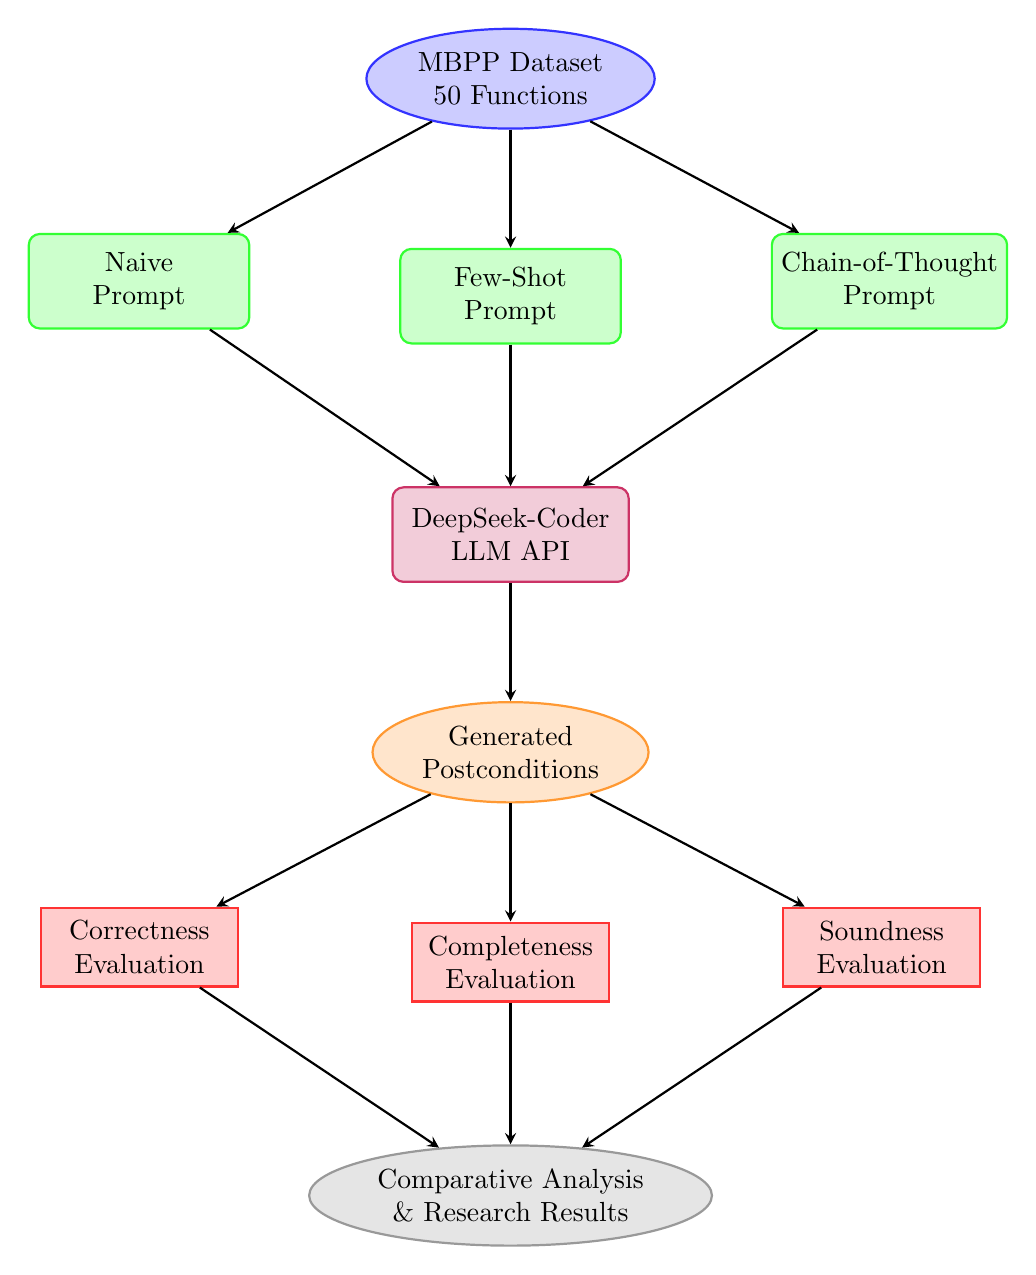
\begin{tikzpicture}[
    node distance=1.8cm,
    auto,
    >=stealth,
    every node/.style={align=center}
]
    % Define styles
    \tikzstyle{input} = [ellipse, minimum width=3cm, minimum height=1.2cm, text centered, draw=blue!80, fill=blue!20, thick]
    \tikzstyle{process} = [rectangle, rounded corners, minimum width=2.8cm, minimum height=1.2cm, text centered, draw=green!80, fill=green!20, thick]
    \tikzstyle{llm} = [rectangle, rounded corners, minimum width=3cm, minimum height=1.2cm, text centered, draw=purple!80, fill=purple!20, thick]
    \tikzstyle{output} = [ellipse, minimum width=3cm, minimum height=1.2cm, text centered, draw=orange!80, fill=orange!20, thick]
    \tikzstyle{evaluation} = [rectangle, minimum width=2.5cm, minimum height=1cm, text centered, draw=red!80, fill=red!20, thick]
    \tikzstyle{final} = [ellipse, minimum width=3.2cm, minimum height=1.2cm, text centered, draw=gray!80, fill=gray!20, thick]
    \tikzstyle{arrow} = [thick, ->, >=stealth]
    
    % Input
    \node [input] (dataset) {MBPP Dataset\\50 Functions};
    
    % Three prompting strategies in a row
    \node [process, below left=1.5cm and 2cm of dataset] (naive) {Naive\\Prompt};
    \node [process, below=1.5cm of dataset] (fewshot) {Few-Shot\\Prompt};
    \node [process, below right=1.5cm and 2cm of dataset] (cot) {Chain-of-Thought\\Prompt};
    
    % LLM processing
    \node [llm, below=1.8cm of fewshot] (llm) {DeepSeek-Coder\\LLM API};
    
    % Generated postconditions
    \node [output, below=1.5cm of llm] (postconds) {Generated\\Postconditions};
    
    % Three evaluation methods in a row
    \node [evaluation, below left=1.5cm and 2.2cm of postconds] (correctness) {Correctness\\Evaluation};
    \node [evaluation, below=1.5cm of postconds] (completeness) {Completeness\\Evaluation};
    \node [evaluation, below right=1.5cm and 2.2cm of postconds] (soundness) {Soundness\\Evaluation};
    
    % Final results
    \node [final, below=1.8cm of completeness] (results) {Comparative Analysis\\\& Research Results};
    
    % Arrows from dataset to prompting strategies
    \draw [arrow] (dataset) -- (naive);
    \draw [arrow] (dataset) -- (fewshot);
    \draw [arrow] (dataset) -- (cot);
    
    % Arrows from prompting strategies to LLM
    \draw [arrow] (naive) -- (llm);
    \draw [arrow] (fewshot) -- (llm);
    \draw [arrow] (cot) -- (llm);
    
    % Arrow from LLM to postconditions
    \draw [arrow] (llm) -- (postconds);
    
    % Arrows from postconditions to evaluation methods
    \draw [arrow] (postconds) -- (correctness);
    \draw [arrow] (postconds) -- (completeness);
    \draw [arrow] (postconds) -- (soundness);
    
    % Arrows from evaluation methods to results
    \draw [arrow] (correctness) -- (results);
    \draw [arrow] (completeness) -- (results);
    \draw [arrow] (soundness) -- (results);
    
\end{tikzpicture}
\end{center}

\section{Technology Stack and Implementation Details}

\subsection{Core Technology Selection}
\begin{itemize}[itemsep=0pt]
    \item \textbf{Programming Language}: Python 3.10+ (for extensive library ecosystem and LLM integration capabilities)
    \item \textbf{LLM Model}: DeepSeek-Coder (for consistent evaluation baseline)
    \item \textbf{Testing Framework}: Pytest + Hypothesis (property-based testing implementation)
    \item \textbf{Mutation Testing}: Mutmut (systematic mutation generation and analysis)
    \item \textbf{Static Analysis}: Python AST library (postcondition parsing and validation)
    \item \textbf{Data Analysis}: Pandas, Seaborn, Matplotlib (statistical analysis and visualization)
    \item \textbf{Version Control}: Git with collaborative branching strategy
\end{itemize}

\subsection{Development Environment and Infrastructure}
The project employs a \textbf{containerized development approach} using Docker for environment consistency across team members. CI/CD pipeline integration ensures automated testing and code quality maintenance throughout development cycles.

\section{Project Timeline and Milestones}

\subsection{8-Week Development Schedule}

\begin{center} % center the chart
% paste after \usepackage{pgfgantt}
\ganttset{
  group left shift=0,     
  group right shift=0,       
  group top shift=0,    
  group height=.6,    
  bar height=.36,          
  group peaks tip position=0 
}

\begin{ganttchart}[
    x unit=1.4cm,                % controls overall chart width -> helps centering
    y unit chart=0.8cm,
    canvas/.append style={fill=none, draw=black!5, line width=.75pt},
    hgrid style/.style={draw=black!5, line width=.75pt},
    vgrid={*1{draw=black!5, line width=.75pt}},
    today=0,
    today rule/.style={
        draw=black!64,
        dash pattern=on 3.5pt off 4.5pt,
        line width=1.5pt
    },
    today label font=\small\bfseries,
    title height=1,
    title/.style={draw=none, fill=none},
    title label font=\bfseries\footnotesize,
    include title in canvas=false,
    bar label font=\mdseries\small\color{black!70},
    bar label node/.append style={left=2cm},
    bar/.append style={draw=none, fill=black!63},
    group height=.5
]{1}{8}

\gantttitlelist{1,...,8}{1} \\[grid]

\node[anchor=east,font=\bfseries\small] at ($(current bounding box.north west)+(-2.0cm,-0.73cm)$) {WEEKS};


% Phase 1: Setup & Design (Blue)
\ganttgroup[group/.append style={fill=phase1color}]{Phase 1: Setup \& Design}{1}{2} \\
\ganttbar[bar/.append style={fill=phase1color!80}]{Environment Setup}{1}{1} \\
\ganttbar[bar/.append style={fill=phase1color!80}]{Architecture Design}{1}{2} \\[grid]

% Phase 2: Core Development (Green)
\ganttgroup[group/.append style={fill=phase2color}]{Phase 2: Core Development}{2}{5} \\
\ganttbar[bar/.append style={fill=phase2color!80}]{Data Pipeline}{2}{3} \\
\ganttbar[bar/.append style={fill=phase2color!80}]{LLM Integration}{2}{4} \\
\ganttbar[bar/.append style={fill=phase2color!80}]{Evaluation Framework}{3}{5} \\[grid]

% Phase 3: Testing & Analysis (Yellow)
\ganttgroup[group/.append style={fill=phase3color}]{Phase 3: Testing \& Analysis}{5}{7} \\
\ganttbar[bar/.append style={fill=phase3color!80}]{System Integration}{5}{6} \\
\ganttbar[bar/.append style={fill=phase3color!80}]{Evaluation Execution}{6}{7} \\[grid]

% Phase 4: Results & Reporting (Red)
\ganttgroup[group/.append style={fill=phase4color}]{Phase 4: Results \& Reporting}{7}{8} \\
\ganttbar[bar/.append style={fill=phase4color!80}]{Data Analysis}{7}{8} \\
\ganttbar[bar/.append style={fill=phase4color!80}]{Final Report}{7}{8} \\

\end{ganttchart}
\end{center}

\subsection{Detailed Milestone Breakdown}

\textbf{Weeks 1-2: Foundation Phase}
\begin{itemize}[itemsep=0pt]
    \item Development environment standardization and Docker containerization
    \item MBPP dataset acquisition, analysis, and preprocessing pipeline
    \item System architecture finalization and interface specification
    \item DeepSeek-Coder API integration and authentication setup
\end{itemize}

\textbf{Weeks 3-4: Core Implementation Phase}
\begin{itemize}[itemsep=0pt]
    \item Three prompting strategies implementation and testing
    \item Property-based testing framework development
    \item Mutation analysis pipeline construction
    \item Static analysis module for hallucination detection
\end{itemize}

\textbf{Weeks 5-6: Integration and Validation Phase}
\begin{itemize}[itemsep=0pt]
    \item End-to-end system integration and interface testing
    \item Pilot evaluation runs with subset of functions
    \item Performance optimization and error handling implementation
    \item Quality assurance and unit testing completion
\end{itemize}

\textbf{Weeks 7-8: Evaluation and Analysis Phase}
\begin{itemize}[itemsep=0pt]
    \item Full-scale evaluation execution across all 50 functions
    \item Statistical analysis and visualization generation
    \item Comparative analysis report compilation
    \item Final presentation preparation and documentation
\end{itemize}

\subsection{Risk Mitigation and Contingency Planning}
Key identified risks include LLM API rate limiting, mutation testing complexity, and evaluation framework scalability. Mitigation strategies include API quota management, simplified mutation strategies as fallbacks, and performance profiling for optimization opportunities.

\section{Expected Outcomes and Success Metrics}

The project's success will be measured through \textbf{quantitative comparative analysis} demonstrating statistically significant differences between prompting strategies across the three evaluation dimensions. Expected deliverables include a reproducible evaluation pipeline, comprehensive statistical analysis, and actionable insights for LLM-assisted software verification practices.

The research contribution extends beyond immediate course requirements, potentially informing future automated verification research and establishing benchmarks for LLM postcondition generation evaluation.

\end{document}